% Options for packages loaded elsewhere
\PassOptionsToPackage{unicode}{hyperref}
\PassOptionsToPackage{hyphens}{url}
%
\documentclass[
  doc, donotrepeattitle,floatsintext]{apa7}
\usepackage{amsmath,amssymb}
\usepackage{lmodern}
\usepackage{iftex}
\ifPDFTeX
  \usepackage[T1]{fontenc}
  \usepackage[utf8]{inputenc}
  \usepackage{textcomp} % provide euro and other symbols
\else % if luatex or xetex
  \usepackage{unicode-math}
  \defaultfontfeatures{Scale=MatchLowercase}
  \defaultfontfeatures[\rmfamily]{Ligatures=TeX,Scale=1}
\fi
% Use upquote if available, for straight quotes in verbatim environments
\IfFileExists{upquote.sty}{\usepackage{upquote}}{}
\IfFileExists{microtype.sty}{% use microtype if available
  \usepackage[]{microtype}
  \UseMicrotypeSet[protrusion]{basicmath} % disable protrusion for tt fonts
}{}
\makeatletter
\@ifundefined{KOMAClassName}{% if non-KOMA class
  \IfFileExists{parskip.sty}{%
    \usepackage{parskip}
  }{% else
    \setlength{\parindent}{0pt}
    \setlength{\parskip}{6pt plus 2pt minus 1pt}}
}{% if KOMA class
  \KOMAoptions{parskip=half}}
\makeatother
\usepackage{xcolor}
\usepackage{graphicx}
\makeatletter
\def\maxwidth{\ifdim\Gin@nat@width>\linewidth\linewidth\else\Gin@nat@width\fi}
\def\maxheight{\ifdim\Gin@nat@height>\textheight\textheight\else\Gin@nat@height\fi}
\makeatother
% Scale images if necessary, so that they will not overflow the page
% margins by default, and it is still possible to overwrite the defaults
% using explicit options in \includegraphics[width, height, ...]{}
\setkeys{Gin}{width=\maxwidth,height=\maxheight,keepaspectratio}
% Set default figure placement to htbp
\makeatletter
\def\fps@figure{htbp}
\makeatother
\setlength{\emergencystretch}{3em} % prevent overfull lines
\providecommand{\tightlist}{%
  \setlength{\itemsep}{0pt}\setlength{\parskip}{0pt}}
\setcounter{secnumdepth}{-\maxdimen} % remove section numbering
% Make \paragraph and \subparagraph free-standing
\ifx\paragraph\undefined\else
  \let\oldparagraph\paragraph
  \renewcommand{\paragraph}[1]{\oldparagraph{#1}\mbox{}}
\fi
\ifx\subparagraph\undefined\else
  \let\oldsubparagraph\subparagraph
  \renewcommand{\subparagraph}[1]{\oldsubparagraph{#1}\mbox{}}
\fi
\newlength{\cslhangindent}
\setlength{\cslhangindent}{1.5em}
\newlength{\csllabelwidth}
\setlength{\csllabelwidth}{3em}
\newlength{\cslentryspacingunit} % times entry-spacing
\setlength{\cslentryspacingunit}{\parskip}
\newenvironment{CSLReferences}[2] % #1 hanging-ident, #2 entry spacing
 {% don't indent paragraphs
  \setlength{\parindent}{0pt}
  % turn on hanging indent if param 1 is 1
  \ifodd #1
  \let\oldpar\par
  \def\par{\hangindent=\cslhangindent\oldpar}
  \fi
  % set entry spacing
  \setlength{\parskip}{#2\cslentryspacingunit}
 }%
 {}
\usepackage{calc}
\newcommand{\CSLBlock}[1]{#1\hfill\break}
\newcommand{\CSLLeftMargin}[1]{\parbox[t]{\csllabelwidth}{#1}}
\newcommand{\CSLRightInline}[1]{\parbox[t]{\linewidth - \csllabelwidth}{#1}\break}
\newcommand{\CSLIndent}[1]{\hspace{\cslhangindent}#1}
\ifLuaTeX
\usepackage[bidi=basic]{babel}
\else
\usepackage[bidi=default]{babel}
\fi
\babelprovide[main,import]{english}
% get rid of language-specific shorthands (see #6817):
\let\LanguageShortHands\languageshorthands
\def\languageshorthands#1{}
% Manuscript styling
\usepackage{upgreek}
\captionsetup{font=singlespacing,justification=justified}

% Table formatting
\usepackage{longtable}
\usepackage{lscape}
% \usepackage[counterclockwise]{rotating}   % Landscape page setup for large tables
\usepackage{multirow}		% Table styling
\usepackage{tabularx}		% Control Column width
\usepackage[flushleft]{threeparttable}	% Allows for three part tables with a specified notes section
\usepackage{threeparttablex}            % Lets threeparttable work with longtable

% Create new environments so endfloat can handle them
% \newenvironment{ltable}
%   {\begin{landscape}\centering\begin{threeparttable}}
%   {\end{threeparttable}\end{landscape}}
\newenvironment{lltable}{\begin{landscape}\centering\begin{ThreePartTable}}{\end{ThreePartTable}\end{landscape}}

% Enables adjusting longtable caption width to table width
% Solution found at http://golatex.de/longtable-mit-caption-so-breit-wie-die-tabelle-t15767.html
\makeatletter
\newcommand\LastLTentrywidth{1em}
\newlength\longtablewidth
\setlength{\longtablewidth}{1in}
\newcommand{\getlongtablewidth}{\begingroup \ifcsname LT@\roman{LT@tables}\endcsname \global\longtablewidth=0pt \renewcommand{\LT@entry}[2]{\global\advance\longtablewidth by ##2\relax\gdef\LastLTentrywidth{##2}}\@nameuse{LT@\roman{LT@tables}} \fi \endgroup}

% \setlength{\parindent}{0.5in}
% \setlength{\parskip}{0pt plus 0pt minus 0pt}

% Overwrite redefinition of paragraph and subparagraph by the default LaTeX template
% See https://github.com/crsh/papaja/issues/292
\makeatletter
\renewcommand{\paragraph}{\@startsection{paragraph}{4}{\parindent}%
  {0\baselineskip \@plus 0.2ex \@minus 0.2ex}%
  {-1em}%
  {\normalfont\normalsize\bfseries\itshape\typesectitle}}

\renewcommand{\subparagraph}[1]{\@startsection{subparagraph}{5}{1em}%
  {0\baselineskip \@plus 0.2ex \@minus 0.2ex}%
  {-\z@\relax}%
  {\normalfont\normalsize\itshape\hspace{\parindent}{#1}\textit{\addperi}}{\relax}}
\makeatother

% \usepackage{etoolbox}
\makeatletter
\patchcmd{\HyOrg@maketitle}
  {\section{\normalfont\normalsize\abstractname}}
  {\section*{\normalfont\normalsize\abstractname}}
  {}{\typeout{Failed to patch abstract.}}
\patchcmd{\HyOrg@maketitle}
  {\section{\protect\normalfont{\@title}}}
  {\section*{\protect\normalfont{\@title}}}
  {}{\typeout{Failed to patch title.}}
\makeatother

\usepackage{xpatch}
\makeatletter
\xapptocmd\appendix
  {\xapptocmd\section
    {\addcontentsline{toc}{section}{\appendixname\ifoneappendix\else~\theappendix\fi\\: #1}}
    {}{\InnerPatchFailed}%
  }
{}{\PatchFailed}
\keywords{Metascience, Sample size planning, Positivity rates, Effect size
\newline \newline \hspace*{\fill} \textcolor{orange}{\textbf{\emph{PREPRINT - NOT PEER-REVIEWED}}} \hspace*{\fill}
\newline \newline \emph{Please cite as}: McKay, B., Corson, A., Vinh, MA., Jeyarajan, G., Tandon, C., Brooks, H., Hubley, J., \& Carter, M.J. (2022). Low prevalence of a priori power analyses in motor behavior research. \emph{SportR$\chi$iv}
}
\usepackage{csquotes}
\usepackage{pdflscape}
\usepackage{setspace}
\raggedbottom
\renewcommand\author[1]{}
\renewcommand\affiliation[1]{}
\authorsnames[1, 2, 2, 3, 3, 2, 2, 1]{Brad McKay, Abbey Corson, Mary-Anne Vinh, Gianna Jeyarajan, Chitrini Tandon, Hugh Brooks, Julie Hubley, Michael J. Carter\vspace{2ex}}
\authorsaffiliations{{Department of Kinesiology, McMaster University}, {School of Human Kinetics, University of Ottawa}, {School of Interdisciplinary Sciences, McMaster University}}
\ifLuaTeX
  \usepackage{selnolig}  % disable illegal ligatures
\fi
\IfFileExists{bookmark.sty}{\usepackage{bookmark}}{\usepackage{hyperref}}
\IfFileExists{xurl.sty}{\usepackage{xurl}}{} % add URL line breaks if available
\urlstyle{same} % disable monospaced font for URLs
\hypersetup{
  pdftitle={Low prevalence of a priori power analyses in motor behavior research},
  pdflang={en-EN},
  pdfkeywords={Metascience, Sample size planning, Positivity rates, Effect size
\newline \newline \hspace*{\fill} \textcolor{orange}{\textbf{\emph{PREPRINT - NOT PEER-REVIEWED}}} \hspace*{\fill}
\newline \newline \emph{Please cite as}: McKay, B., Corson, A., Vinh, MA., Jeyarajan, G., Tandon, C., Brooks, H., Hubley, J., \& Carter, M.J. (2022). Low prevalence of a priori power analyses in motor behavior research. \emph{SportR$\chi$iv}},
  hidelinks,
  pdfcreator={LaTeX via pandoc}}

\title{Low prevalence of \emph{a priori} power analyses in motor behavior research}
\author{\phantom{0}}
\date{}


\shorttitle{Power analyses in motor behavior}

\authornote{

\vspace{-0.5cm}

\noindent \addORCIDlink{Brad McKay}{0000-0002-7408-2323} \newline
\noindent \addORCIDlink{Michael J. Carter}{0000-0002-0675-4271} \vspace{2ex} \newline
\noindent Data and code: \url{https://osf.io/wsdpv/} \vspace{2ex} \newline
\noindent \textbf{Corresponding authors:} Brad McKay (\href{mailto:bradmckay8@gmail.com}{\nolinkurl{bradmckay8@gmail.com}}; \href{mailto:mckayb9@mcmaster.ca}{\nolinkurl{mckayb9@mcmaster.ca}}) and Michael J. Carter (\href{mailto:cartem11@mcmaster.ca}{\nolinkurl{cartem11@mcmaster.ca}}; \href{mailto:motorlab@mcmaster.ca}{\nolinkurl{motorlab@mcmaster.ca}})

}

\affiliation{\phantom{0}}

\abstract{%
\emph{A priori} power analyses can be used to ensure studies are unlikely to miss interesting effects. Recent metascience has suggested that kinesiology research may be underpowered and selectively reported. Here, we examined whether power analyses were currently being leveraged to ensure informative studies in the motor behavior research. We reviewed every article published in the \emph{Journal of Motor Learning and Development}, the \emph{Journal of Motor Behavior}, and \emph{Human Movement Science} between January 2019 and June 2021. Our results revealed that power analyses were reported in 13\% of all studies (\emph{k} = 636) that tested a hypothesis. Yet, no study in the sample targeted the smallest effect size of interest. Most studies with a power analysis instead relied on estimates from previous studies, pilot studies, or benchmarks to determine the effect size of interest. Studies in this sample without a power analysis reported support for their main hypothesis 85\% of the time, while studies with a power analysis found support 76\% of the time. The median sample sizes were \emph{n} = 17.5 without a power analysis and \emph{n} = 16 with a power analysis, suggesting the typical study design in our sample was underpowered for all but the largest plausible effect size. At present, power analyses are not being used to optimize the informativeness of motor behavior studies; a trend that likely extends to other kinesiology subdisciplines. Adoption of this simple and widely recommended practice may greatly enhance the credibility of the motor behavior literature and kinesiology research in general.
}



\begin{document}
\maketitle

Motor behavior research frequently involves proposing hypotheses and subjecting them to statistical tests. The probability that a statistical test will correctly reject the null hypothesis, conditional on a true effect of a given size and an accepted rate of false-positive results, is called power (Cohen, 1962, 1988; Neyman, 1937, 1942). Power should be a central concern for statistical hypothesis testers with finite resources and the journals that publish their results. For researchers, power calculations are useful when designing studies to optimize the use of resources, and especially for avoiding studies that have a low probability of producing informative results. For journals, the range of effects a study has the power to rule out is an indication of how potentially informative that study was \emph{a priori}. Unfortunately, power analyses can also be misleading. Power can be seriously overestimated by the wrong parameters---many of which are entirely based on the researcher's judgment. To conduct a power analysis at least four parameters are required: the design of the study, the size of the assumed effect, the frequency of false-positives, and the frequency of false-negatives. Although each of these specifications should be justified (Lakens et al., 2018; Lakens, 2022b), researchers often rely on conventions. For example, false-positive and false-negative rates have conventionally been set at 5\% and 20\%, respectively (Cohen, 1988). Many researchers and journals may consider false-negative rates of 10\% or 5\% more appropriate, but this consideration should be made thoughtfully (see Lakens, 2022b for a discussion).

Standardized effect sizes also have conventional benchmarks that researchers may rely on when designing studies. Recent metascience suggests doing so is likely to result in underpowered research designs in practice (Lovakov \& Agadullina, 2021). Instead of relying on benchmarks, some researchers may base their effect size target on a previous study or the results of a pilot study. However, large multi-lab replication studies have revealed that original studies may overestimate the true effect of an independent variable by 100\% to 400\% (Klein et al., 2018; Open Science Collaboration, 2015). Pilot studies are often even less helpful, as they tend to be smaller than published experiments so their estimates are even more imprecise (Albers \& Lakens, 2018; Kraemer et al., 2006; Lakens \& Evers, 2014). When available, meta-analyses provide an effect size estimate based on the aggregation of available data. However, selective reporting of results can distort meta-analytic estimates and it can be difficult to correct for reporting bias (Carter et al., 2019; Thornton \& Lee, 2000). Nevertheless, estimates that have been corrected for reporting bias are more accurate than naïve random effects estimates and should be used when available (Carter et al., 2019).

A better strategy for choosing the effect size for an \emph{a priori} power analysis does not rely on mean estimates and instead the researcher specifies their smallest effect size of interest (Lakens, 2022b). If a researcher targeting 80\% power estimates an effect is \emph{d} = .5 but would still be interested if it was \emph{d} = .2, they will miss their smallest effect size of interest 80\% of the time. Instead of powering for the expected effect, researchers that power for their smallest effect size of interest guarantee their study design will not be underpowered for interesting effects. Researchers can extend this strategy to maximize the informativeness of their studies by making one-tailed predictions with 95\% power. In this situation, null results are significantly smaller than the smallest effect size of interest. Studies designed this way may help prevent distortion from selection bias as both positive and negative results can be interpreted as significant.

Given the potential for power analyses to enhance the inferential value of studies and the myriad suboptimal strategies that may be employed, we chose to investigate the proportion of recent studies where motor behavior scientists reported a power analysis and their justification for their selected effect size. We focused on motor behavior research as recent meta-analyses have reported evidence of both underpowered research and substantial reporting bias in motor learning and sports science (Lohse et al., 2016; McKay et al., 2022, in-press; Mesquida et al., 2022). For example, a meta-analysis of the self-controlled motor learning literature estimated the average power of all studies conducted was 6\%, while 48\% of studies reported significant results on the focal measure (McKay et al., in-press). Other studies have estimated average power ranging from 20\% (McKay et al., 2022) to 50\% (Mesquida et al., 2022), with significant indications of reporting bias. The combination of low power and significance-based selective reporting is pernicious to the accumulation of scientific evidence. Statistically significant results in studies with low power are likely to substantially overestimate the effect of the independent variable. When power dips below 10\%, significant results in the wrong direction become increasingly likely (Gelman \& Carlin, 2014).

If motor behavior research does not currently report power analyses---especially for the smallest effect size of interest---then future adoption of these best practices could potentially address issues of low power and selective reporting. Investigating this possibility, we examined the prevalence of \emph{a priori} power analyses in three motor behavior journals, the justifications used for effect size assumptions, and their association with studies finding positive results. The goal of this study was descriptive. Our main purpose was simply to understand the current use of power analyses in the motor behavior literature. However, we did posit several exploratory hypotheses. We predicted that studies with a power analysis would have a different rate of positive results from studies without a power analysis. However, due to potential selection effects we did not speculate about the direction of this difference \emph{a priori}. We predicted that some justifications would differ in the frequency of positive results, with pilot studies being especially unsuccessful. We also predicted that differences in targeted power would be associated with different positivity rates given the primary function of a power analysis. Finally, we predicted that there would be a difference in the sample size obtained by studies that conducted a power analysis compared to those that did not, again without speculating about the direction.

\hypertarget{methods}{%
\section{Methods}\label{methods}}

Our design and analysis plan was preregistered after piloting our methods on a subsample of 40 papers. The preregistration, materials, data, and code from this study is available here: \url{https://osf.io/wsdpv/}.

\hypertarget{power}{%
\subsection{Power}\label{power}}

Calculating \emph{a priori} power for this study required estimating the final sample size and proportion of studies that would include a power analysis. Based on the pilot sample of articles, we estimated that the total number of studies we would extract would be approximately 500. The actual number was 636. We reasoned that if 10\% of those studies included a power analysis, we would have 50 studies with power analyses and 450 studies without power analyses in our sample. The actual numbers were 13\%, 85 and 551. Based on our rough estimates, we conducted simulations to estimate our power to detect differences in positive result rates of various plausible sizes. We based our expected positive results rate in studies without power analyses on estimates for psychology overall at 91.5\% (Fanelli, 2010). We observed that, if our estimates were accurate, we would have 90\% power to detect a difference of 16.5\%, or a positive result rate of 75\% in experiments with power analyses. Similarly, we estimated we would have 80\% power to identify a positive result rate of 77.7\% as significantly different. Unfortunately, if our estimated group sizes were accurate, we would have had low power (32\%) to detect our smallest effect size of interest (6\%). Given the actual sample sizes we observed, we had even greater power than planned to observe the effects we considered.

\hypertarget{sample}{%
\subsection{Sample}\label{sample}}

All articles published in the \emph{Journal of Motor Learning and Development}, \emph{Human Movement Science}, and the \emph{Journal of Motor Behavior} between January 2019 to June 2021 were uploaded to Covidence systematic review software and screened for inclusion (Figure \ref{fig:fig1}). In total, 704 articles were reviewed. To be included in the analysis, studies were required to meet the following criteria: a) must be a primary study, b) must test a hypothesis, including the null hypothesis, c) there must be sufficient information available to adequately evaluate the criteria, and d) we must have access to the full-text. From the original 704 articles, 607 articles included at least one study that met the inclusion criteria and were included in the final analysis. Ninety-seven articles were excluded from the analysis for the following reasons: a) the studies were not primarily quantitative (63 studies), b) the studies made no hypothesis (27 studies), or there was insufficient information or a faulty DOI to assess the paper (7). The 607 included articles contributed a total of 636 eligible studies to the analysis.

\pagebreak

\begin{figure}

{\centering 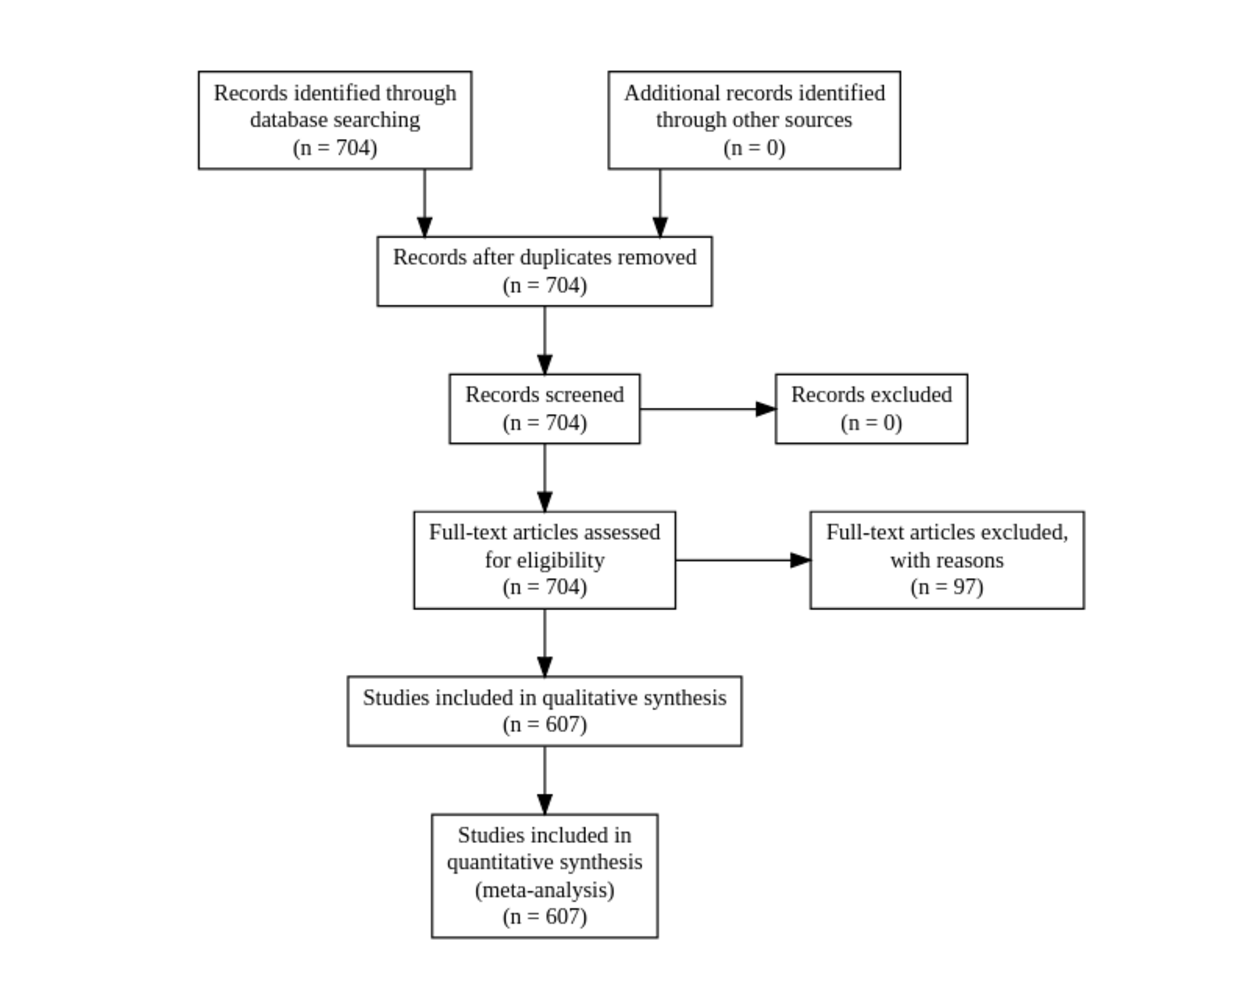
\includegraphics{../../figs/fig1} 

}

\caption{PRISMA flow diagram.}\label{fig:fig1}
\end{figure}



\pagebreak

\hypertarget{procedures}{%
\subsection{Procedures}\label{procedures}}

Data extraction was conducted by an extraction team of eight researchers. Two independent researchers evaluated each article in Covidence, with a third researcher resolving any conflicts. In situations where a member of the extraction team encountered a challenging item, the member flagged the study on Covidence for the items to be extracted and the consensus decision to be made by the first author (\emph{N} = 40). We extracted data for 11 items, which are outlined in Table \ref{tab:table1}. For Item 5, determining whether the authors of a study concluded the results supported their hypothesis involved two steps. First, the primary hypothesis of a study was identified, either because the authors specified the hypothesis as primary or it was the first independent hypothesis reported. When hypotheses were listed with multiple components, support for any component was considered support for the hypothesis. Any hypothesis explicitly labeled as secondary was not considered. Second, the interpretation of the results by the authors was examined. We coded support for hypotheses based on the interpretations in each paper, not based on our own criteria. Thus, if the authors predicted no effect of an independent variable, observed null results, and then concluded the results supported their hypothesis, we coded this as support for the hypothesis.

\begin{table}

\caption{\label{tab:table1}Elements of the data extraction process and the corresponding action the researchers performed.}
\fontsize{10}{12}\selectfont
\begin{tabular}[t]{>{\raggedright\arraybackslash}p{21em}>{\raggedright\arraybackslash}p{20em}}
\toprule
Item & Action\\
\midrule
1. Did the study meet the inclusion criteria? & Yes or No, and provide reason.\\
\addlinespace
2. Did the authors report a power analysis? & Yes or No.\\
\addlinespace
3. Hypothesis quote. & Copy pasted quote of the hypotheses.\\
\addlinespace
4. Results quote. & Copy pasted quote of the results interpretation\\
\addlinespace
5. Did the authors conclude support for any of the main hypotheses? & Yes or No.\\
\addlinespace
6. Sample size. & Calculate average per group.\\
\addlinespace
7. Power analysis effect type. & Select from a list.\\
\addlinespace
8. Power analysis effect estimate. & Report the effect size used for the analysis.\\
\addlinespace
9. Power analysis effect converted to Cohen's d. & Perform conversion whenever possible.\\
\addlinespace
10. Effect size justification. & Select from a list.\\
\addlinespace
11. Power estimate from the power analysis. & Report value.\\
\bottomrule
\end{tabular}
\end{table}

\hypertarget{statistical-analysis}{%
\subsection{Statistical Analysis}\label{statistical-analysis}}

To evaluate the overall prevalence of power analyses in the sampled literature, we calculated the percentage of all studies in our sample that conducted a power analysis:
\[\frac{studies\, with\, power\, analysis}{studies\, with\, power\, analysis\, + studies\, without\, power\, analysis} \times 100\]
We used a two-sided proportion test to assess whether the rate of positive results in studies with a power analysis was significantly different than in studies without a power analysis. We also tested whether the difference in positive result rates was statistically smaller than our smallest effect size of interest (6\%) using an equivalence test for proportions.

We calculated the percentage of studies that conducted a power analysis with a) each effect justification and b) each power target. A two-sided, six sample proportion test was conducted to test whether at least two different effect size justifications in power analyses led to different rates of positive results. A two-sided, 11-sample proportion test was conducted to test whether at least two power targets resulted in a different rate of positive results. Lastly, we conducted a two-tailed Welch's \emph{t}-test to determine whether studies with power analyses had different sample sizes compared to studies without power analyses. Given the data were highly skewed, we also conducted a sensitivity analysis using a shift function (Rousselet et al., 2017; Rousselet \& Wilcox, 2020; Wilcox, 2021).

Statistical tests were conducted using R (Version 4.1.2; R Core Team, 2021) and the R-packages \emph{diagramme} (Iannone, 2016), \emph{extrafont} (Version 0.18; Chang, 2022), \emph{kableExtra} (Version 1.3.4; Zhu, 2021, 2021), \emph{papaja} (Version 0.1.0.9999; Aust \& Barth, 2020), \emph{prisma} (Jack O. Wasey, 2019), \emph{rcolorbrewer} (Neuwirth, 2022), \emph{renv} (Version 0.15.5; Ushey, 2022), \emph{rogme} (Version 0.2.1; Rousselet et al., 2017), \emph{rsvg} (Version 2.3.1; Ooms, 2022), \emph{tidyverse} (Version 1.3.1; Wickham et al., 2019), \emph{tinylabels} (Version 0.2.3; Barth, 2022), \emph{toster} (Lakens, 2017), and \emph{waffle} (Version 1.0.1; Rudis \& Gandy, 2019) were used in this project.

\hypertarget{results}{%
\section{Results}\label{results}}

\hypertarget{proportion-of-studies-with-a-power-analysis}{%
\subsection{Proportion of Studies with a Power Analysis}\label{proportion-of-studies-with-a-power-analysis}}

Out of 636 total studies, 85 included a power analysis and 551 did not. Therefore, 13\% of all studies sampled reported the results of a power analysis.

\hypertarget{difference-in-positivity-rates-between-studies-with-and-without-a-power-analysis}{%
\subsection{Difference in Positivity Rates between Studies with and without a Power Analysis}\label{difference-in-positivity-rates-between-studies-with-and-without-a-power-analysis}}

As shown in Figure \ref{fig:fig2}, studies that did not include a power analysis reported finding support for their primary hypothesis 85\% of the time (95\% CI {[}82\%, 88\%{]}), while studies that included a power analysis found support 76\% of the time (95\% CI {[}66\%, 85\%{]}). The difference in positivity rates was not statistically significant, \(\chi^2\)= 3.47, \emph{df} = 1, \emph{p} = .06. The difference is positivity rates was not significantly smaller than our smallest effect size of interest, \emph{Z} = .546, \emph{p} = .71.

\hypertarget{justifications-for-effect-sizes-used-in-power-analyses}{%
\subsection{Justifications for Effect Sizes used in Power Analyses}\label{justifications-for-effect-sizes-used-in-power-analyses}}

The most common justification reported in our sample was to base the expected effect size on a previous study (\emph{n} = 37), accounting for 44\% of all justifications. The second most common justification was to provide no justification at all (\emph{n} = 20), which occurred in 24\% of studies that included a power analysis. Cohen's benchmarks for small, medium, and large effects (\emph{n} = 19) were used in 22\% of studies. Pilot studies (\emph{n} = 9) were used as justification in 11\% of the sample.

\pagebreak

\begin{figure}

{\centering 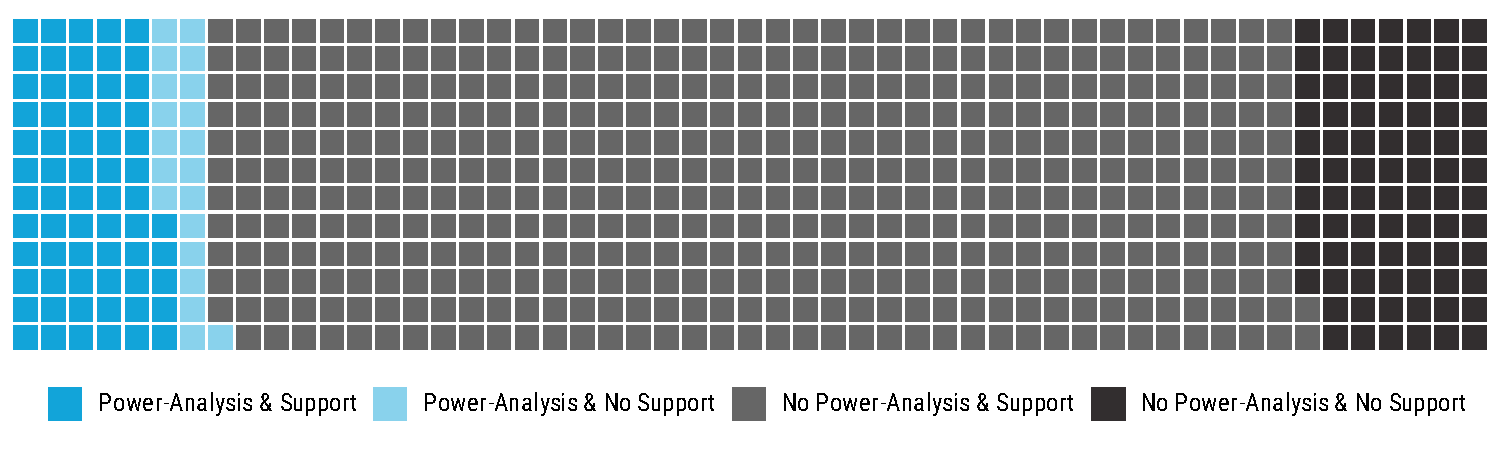
\includegraphics{../../figs/fig2} 

}

\caption{Proportion of studies with (blue) and without (grey) power analyses and whether the authors concluded support for their primary hypotheses. Each square represents a single study in our sample. The majority of studies in our sample did not include a power analysis. The most common combination was ``No Power-Analysis \& Support'' (light grey) while ``Power-Analysis \& No Support'' (light blue) was the least common combination.}\label{fig:fig2}
\end{figure}



\pagebreak

\hypertarget{power-levels-targeted-in-power-analyses}{%
\subsection{Power Levels Targeted in Power Analyses}\label{power-levels-targeted-in-power-analyses}}

The most frequently targeted power was 80\%, which was chosen in 65\% of studies with a power analysis (\emph{n} = 55). The next most common power target was 95\%, accounting for 14\% of all power targets (\emph{n} = 12); followed by 90\% power, occurring in 11\% of power analyses (\emph{n} = 9). Two studies did not state their targeted power and several idiosyncratic power targets (96.7\%, 96\%, 95.33\%, 85\%, 75\%, 70\%, and 20\%) were reported only once.

\hypertarget{difference-in-positivity-rates-as-a-function-of-effect-size-justification}{%
\subsection{Difference in Positivity Rates as a Function of Effect Size Justification}\label{difference-in-positivity-rates-as-a-function-of-effect-size-justification}}

Figure \ref{fig:fig3} illustrates the proportion of positive results for the four effect size justifications we found in our sample. Positivity rates were 100\% for pilot study justification (9/9), 90\% for studies with no justification (18/20), 68\% for studies based on benchmarks (13/19), and 68\% for studies based on previous studies (25/37). There was no significant difference between the positivity rates of any two justifications, \(\chi^2\) = 7.12, \emph{df} = 3, \emph{p} = .068.

\hypertarget{difference-in-positivity-rates-as-a-function-of-target-power}{%
\subsection{Difference in Positivity Rates as a Function of Target Power}\label{difference-in-positivity-rates-as-a-function-of-target-power}}

Studies that targeted 80\% power found support for their hypotheses 68\% of the time (38/56). Studies that aimed for 90\% power found support 100\% of the time (8/8) and studies that aimed for 95\% power found support 75\% of the time (9/12). All studies that set an idiosyncratic power target or no target at all found support for their hypotheses (10/10). There was no significant difference between target power values, \(\chi^2\)= 7.22, \emph{df} = 10, \emph{p} = .70.

\hypertarget{difference-in-sample-size-between-studies-with-and-without-a-power-analysis}{%
\subsection{Difference in Sample Size between Studies with and without a Power Analysis}\label{difference-in-sample-size-between-studies-with-and-without-a-power-analysis}}

Studies that included a power analysis had significantly smaller mean sample sizes (\emph{M} = 21.91) than studies that did not include a power analysis (\emph{M} = 40.98), \emph{t}(624.59)= 3.43, \emph{p} = .001. However, sample sizes were highly skewed---especially among studies without a power analysis. The median sample for those studies (\emph{Mdn} = 17.5) was similar to the sample sizes of studies with a power analysis (\emph{Mdn} = 16). We conducted a shift function as a sensitivity analysis and the results indicated no significant difference in sample size between studies with and without power analyses at any decile of their distributions.

\pagebreak

\begin{figure}

{\centering 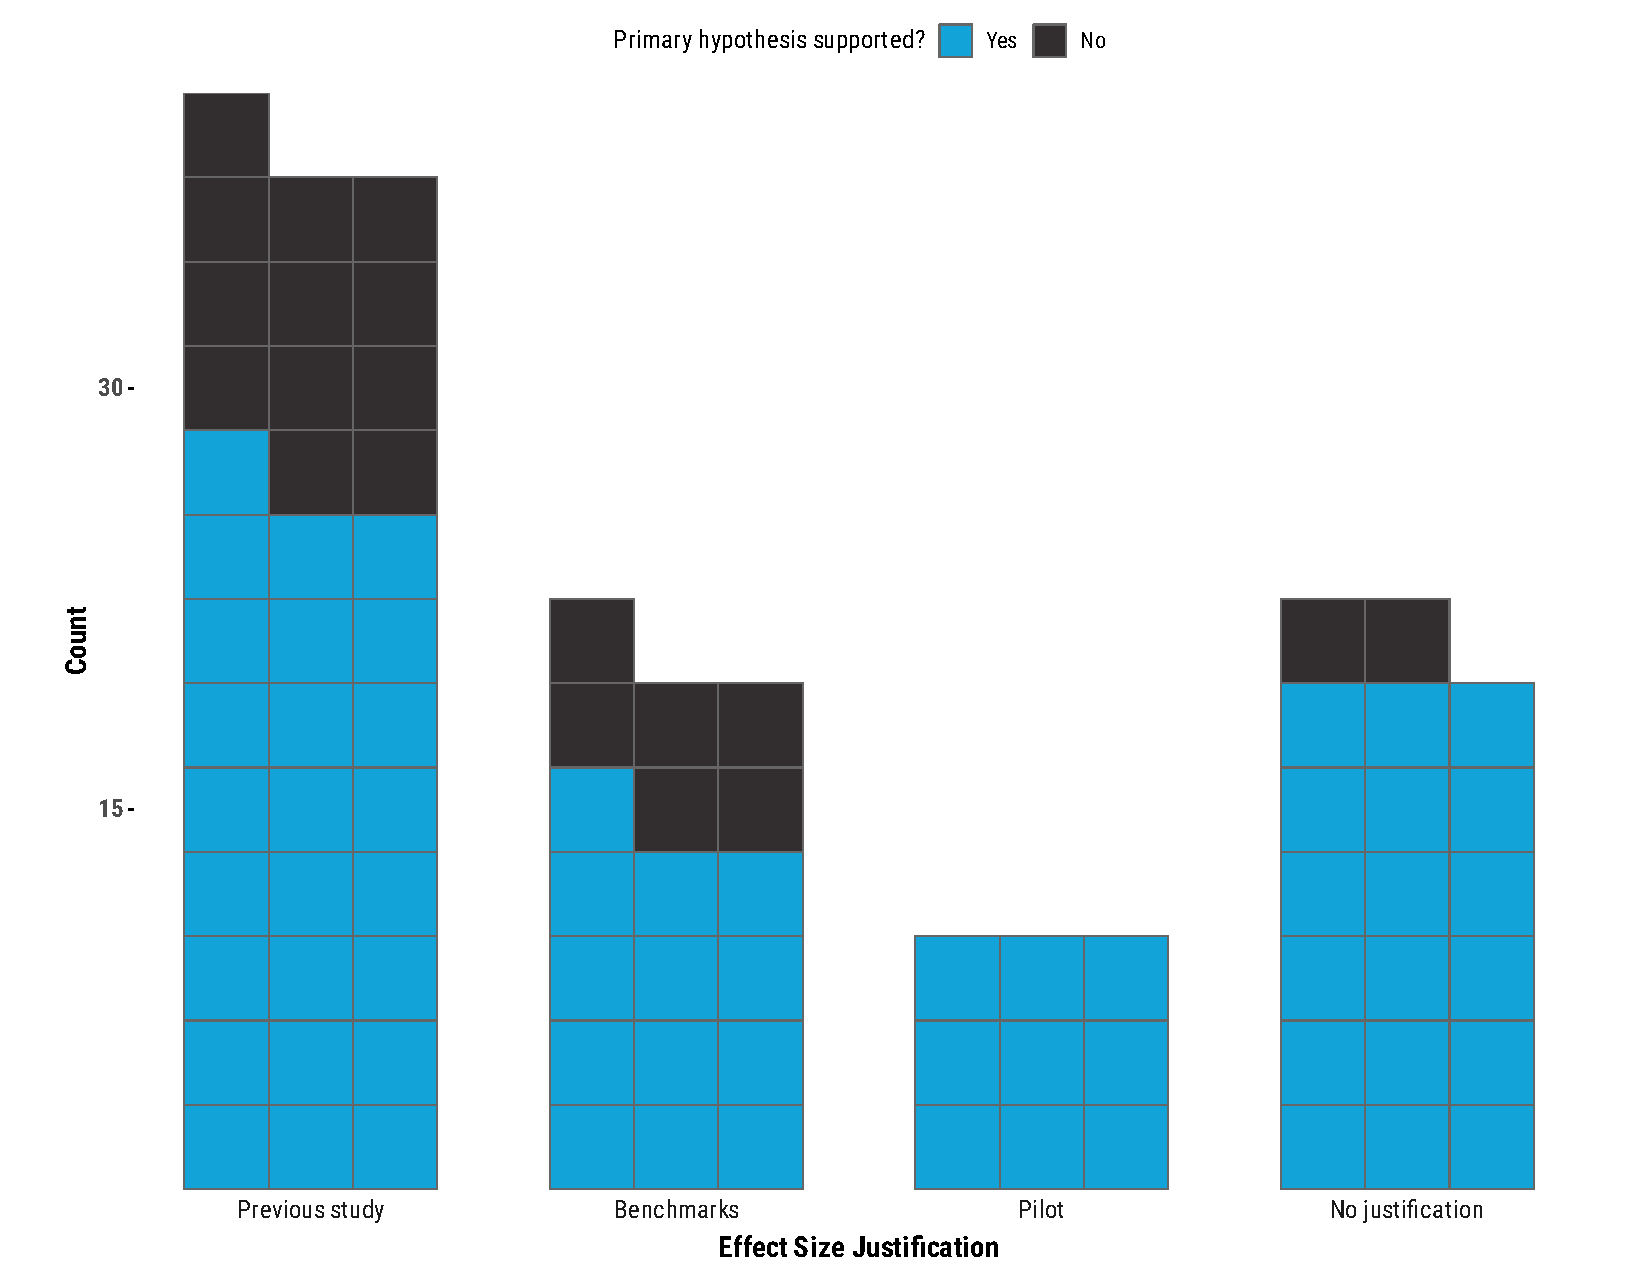
\includegraphics{../../figs/fig3} 

}

\caption{Proportion of studies where authors concluded support (blue) or no support (black) for their primary hypotheses as a function of their effect size justification. Each square represents a single study. Of the list of possible effect size justifications, we only found data for four justifications.}\label{fig:fig3}
\end{figure}



\pagebreak

\hypertarget{discussion}{%
\section{Discussion}\label{discussion}}

The purpose of this study was to investigate how frequently power analyses are reported in motor behavior articles, the justifications used for the effect size estimates, and the relationship between reporting power analyses and reporting positive results. We reviewed every article published in the \emph{Journal of Motor Behavior}, the \emph{Journal of Motor Learning and Development}, and \emph{Human Movement Science} between January 2019 and June 2021 and identified 636 studies that tested a hypothesis. Of those 636 studies, 85 of them included a power analysis (13\%). The rate of positive results was 85\% overall and 76\% when a power analysis was reported. The positive result rate was not significantly different between various effect size justifications or power targets.

Our results suggest that motor behavior research has not yet widely adopted power analyses to inform study design. When power analyses were reported, we observed a range of suboptimal effect size justifications. For example, 63\% of studies that reported a power analysis based their effect size assumption on a previous study, a pilot study, or on effect size benchmarks. Another 24\% of studies provided no justification at all. Each of these justifications (or lack thereof) are undesirable for different reasons. Previous studies---and especially pilot studies---are likely to provide exaggerated or noisy estimates of the unknown true effect. Effect size benchmarks may not match well the typical effect sizes one may find in their respective research area (Lovakov \& Agadullina, 2021). Further, Cohen's (Cohen, 1988) benchmarks differ depending on which analysis is used in a power analysis. A medium effect is over twice as large for a multiple regression analysis as compared to a \emph{t}-test (see Correll et al., 2020 for a discussion with additional examples). Not one study in the sample performed a power analysis based on their smallest effect size of interest. Power analyses can be an effective tool for researchers to ensure their studies are not underpowered, but to do so the smallest effects of interest need to be targeted.

The rate of positive results observed in this study suggest that positive findings are overrepresented in the motor behavior literature. While the studies in our sample reported positive results 84\% of the time, the median per group sample size was \textasciitilde17, which would provide 84\% power to detect \emph{d} = 1.05 with an independent \emph{t}-test or \emph{d} = .76 with a dependent \emph{t}-test. In comparison, the most optimistic estimates for well-known motor behavior phenomena are much smaller. For example, the effect of feedback frequency on motor performance (\emph{d} = .19, McKay et al., 2022), self-controlled practice on retention performance (\emph{d} = .54, McKay et al., in-press), enhanced expectancies on retention performance (\emph{d} = .54, Bacelar et al., in-press), and external focus of attention on retention performance (\emph{d} = .58, Chua et al., 2021). Estimates for the true effects of these phenomena that have been corrected for reporting-bias are markedly smaller, ranging from \emph{d} = 0 to \emph{d} = .25. Assuming the average effects investigated by the studies in our sample were similar to the optimistic estimates for other motor behavior effects, it is likely this literature was underpowered on average and potentially heavily censored.

All three journals that we sampled from either explicitly mention power in their instructions for authors (\emph{Human Movement Science}), or reference JARS (\emph{Journal of Motor Learning and Development}) or CONSORT (\emph{Journal of Motor Behavior}) reporting standards; both of which include power analyses. Therefore, adoption of power analyses targeting interesting effects does not require a policy shift, simply the enforcement of current guidelines. Since no studies in this sample powered for the smallest effect size of interest, if \emph{Human Movement Science}, the \emph{Journal of Motor Behavior}, and/or the \emph{Journal of Motor Learning and Development} enforce their existing guidelines then their future publications will look dramatically different. We believe this is a promising path forward to increase the reliability of motor behavior research and the evidence-based recommendations for coaching and rehabilitation.

\hypertarget{limitations}{%
\subsection{Limitations}\label{limitations}}

The specific designs and test statistics from the studies in our sample were not extracted, so we cannot calculate the estimated average power of the sample. This also complicates the interpretation of sample size differences among studies with and without power analyses. For example, if studies that used within-subjects designs were also more likely to conduct a power analysis, it would make sense that those studies would have smaller samples overall. Within-subjects designs are substantially more powerful than between-subjects, so all other things being equal, studies with within-subjects designs require less participants to be adequately powered.

We do not differentiate between partial and full support for hypotheses, nor did we code for whether the hypothesis was directional, non-directional, or if the null hypothesis was framed as the primary hypothesis in the study. As such, we must be cautious not to regard positivity rate as a direct analogue for implied power. There were studies that predicted no difference between experimental conditions, failed to reject the null hypothesis, and then interpreted the result as supporting their primary hypothesis. While this approach to hypothesis testing is problematic, our goal with this study was to describe the proportions of positive results and power analyses, not to critique the specific methods employed in each study.

\hypertarget{conclusion}{%
\section{Conclusion}\label{conclusion}}

Our results suggest that power analyses targeting the smallest effect size of interest (Lakens, 2022a) have the potential to change the state of the motor behavior literature. Hypothesis tests are the norm in this space, yet power calculations targeting interesting effects are not. It is logical for researchers to plan studies with a high probability of producing informative results and it is consistent with current reporting standards (Appelbaum et al., 2018). Given the recent concern about the reliability of established motor behavior phenomena Mesquida et al. (2022), we believe power analyses have an important role to play in increasing the credibility of our field.

\pagebreak

\hypertarget{author-contributions-credit-taxonomy}{%
\subsection{Author Contributions (CRediT Taxonomy)}\label{author-contributions-credit-taxonomy}}

\noindent Conceptualization: BM, MJC\\
Data curation: BM, MJC\\
Formal analysis: BM\\
Funding acquisition: MJC\\
Investigation: BM, AC, MV, GJ, CT, HB, JH\\
Methodology: BM, MJC\\
Project administration: BM, MJC\\
Software: BM, MJC\\
Supervision: BM, MJC\\
Validation: BM, MJC\\
Visualization: BM, MJC\\
Writing -- original draft: BM, AC, MV, GJ, CT, HB, JH, MJC\\
Writing -- review \& editing: BM, AC, MV, GJ, CT, HB, JH, MJC

\hypertarget{acknowledgements}{%
\subsection{Acknowledgements}\label{acknowledgements}}

\noindent All authors thank Aaron Schwarz and Abigail Morgan for their help with data extraction.

\hypertarget{open-science-practices}{%
\subsection{Open Science Practices}\label{open-science-practices}}

\noindent The preregistration, data, and scripts can be accessed using either of the following links: \url{https://osf.io/wsdpv/} or \url{https://github.com/cartermaclab/proj_power-motor-behaviour}.

\hypertarget{conflicts-of-interest}{%
\subsection{Conflicts of Interest}\label{conflicts-of-interest}}

\noindent All authors declare no conflicts of interest.

\hypertarget{funding}{%
\subsection{Funding}\label{funding}}

\noindent This work was supported by the Natural Sciences and Engineering Research Council (NSERC) of Canada (RGPIN-2018-05589; MJC) and McMaster University (MJC).

\pagebreak

\hypertarget{references}{%
\section{References}\label{references}}

\vspace{2ex}

\hypertarget{refs}{}
\begin{CSLReferences}{1}{0}
\leavevmode\vadjust pre{\hypertarget{ref-Albers2018}{}}%
Albers, C., \& Lakens, D. (2018). When power analyses based on pilot data are biased: Inaccurate effect size estimators and follow-up bias. \emph{Journal of Experimental Social Psychology}, \emph{74}, 187--195.

\leavevmode\vadjust pre{\hypertarget{ref-Appelbaum2018}{}}%
Appelbaum, M., Cooper, H., Kline, R. B., Mayo-Wilson, E., Nezu, A. M., \& Rao, S. M. (2018). Journal article reporting standards for quantitative research in psychology: {The} {APA} {Publications} and {Communications} {Board} task force report. \emph{American Psychologist}, \emph{73}(1), 3. \url{https://doi.org/10.1037/amp0000191}

\leavevmode\vadjust pre{\hypertarget{ref-R-papaja}{}}%
Aust, F., \& Barth, M. (2020). \emph{{papaja}: {Prepare} reproducible {APA} journal articles with {R Markdown}}. \url{https://github.com/crsh/papaja}

\leavevmode\vadjust pre{\hypertarget{ref-Bacelar2022}{}}%
Bacelar, M. F. B., Parma, J. O., Murrah, W. M., \& Miller, M. W. (in-press). Meta-analyzing enhanced expectancies on motor learning: Positive effects but methodological concerns. \emph{International Review of Sport and Exercise Psychology}, 1--30. \url{https://doi.org/10.1080/1750984X.2022.2042839}

\leavevmode\vadjust pre{\hypertarget{ref-R-tinylabels}{}}%
Barth, M. (2022). \emph{{tinylabels}: Lightweight variable labels}. \url{https://cran.r-project.org/package=tinylabels}

\leavevmode\vadjust pre{\hypertarget{ref-Carter2019}{}}%
Carter, E. C., Schönbrodt, F. D., Gervais, W. M., \& Hilgard, J. (2019). Correcting for bias in psychology: A comparison of meta-analytic methods. \emph{Advances in Methods and Practices in Psychological Science}, \emph{2}(2), 115--144. \url{https://doi.org/10.1177/2515245919847196}

\leavevmode\vadjust pre{\hypertarget{ref-R-extrafont}{}}%
Chang, W. (2022). \emph{Extrafont: Tools for using fonts}. \url{https://CRAN.R-project.org/package=extrafont}

\leavevmode\vadjust pre{\hypertarget{ref-Chua2021}{}}%
Chua, L.-K., Jimenez-Diaz, J., Lewthwaite, R., Kim, T., \& Wulf, G. (2021). Superiority of external attentional focus for motor performance and learning: Systematic reviews and meta-analyses. \emph{Psychological Bulletin}, \emph{147}(6), 618.

\leavevmode\vadjust pre{\hypertarget{ref-Cohen1962}{}}%
Cohen, J. (1962). The statistical power of abnormal-social psychological research: A review. \emph{The Journal of Abnormal and Social Psychology}, \emph{65}(3), 145--153. \url{https://doi.org/10.1037/h0045186}

\leavevmode\vadjust pre{\hypertarget{ref-Cohen1988}{}}%
Cohen, J. (1988). \emph{Statistical power analysis for the behavioral sciences} (2nd ed). L. Erlbaum Associates.

\leavevmode\vadjust pre{\hypertarget{ref-Correll2020}{}}%
Correll, J., Mellinger, C., McClelland, G. H., \& Judd, C. M. (2020). Avoid {C}ohen's {``small,''} {``medium,''} and ``large" for power analysis. \emph{Trends in Cognitive Sciences}, \emph{24}(3), 200--207.

\leavevmode\vadjust pre{\hypertarget{ref-Fanelli2010}{}}%
Fanelli, D. (2010). {``Positive''} results increase down the hierarchy of the sciences. \emph{PLOS ONE}, \emph{5}(4), e10068. \url{https://doi.org/10.1371/journal.pone.0010068}

\leavevmode\vadjust pre{\hypertarget{ref-Gelman2014}{}}%
Gelman, A., \& Carlin, J. (2014). Beyond power calculations: Assessing type s (sign) and type m (magnitude) errors. \emph{Perspectives on Psychological Science}, \emph{9}(6), 641--651.

\leavevmode\vadjust pre{\hypertarget{ref-R-diagramme}{}}%
Iannone, R. (2016). \emph{DiagrammeRsvg: Export DiagrammeR graphviz graphs as SVG}. \url{https://CRAN.R-project.org/package=DiagrammeRsvg}

\leavevmode\vadjust pre{\hypertarget{ref-R-prisma}{}}%
Jack O. Wasey. (2019). \emph{PRISMAstatement: Plot flow charts according to the "PRISMA" statement}. \url{https://CRAN.R-project.org/package=PRISMAstatement}

\leavevmode\vadjust pre{\hypertarget{ref-Klein2018}{}}%
Klein, R. A., Vianello, M., Hasselman, F., Adams, B. G., Adams, R. B., Alper, S., Aveyard, M., Axt, J. R., Babalola, M. T., Bahník, Š., Batra, R., Berkics, M., Bernstein, M. J., Berry, D. R., Bialobrzeska, O., Binan, E. D., Bocian, K., Brandt, M. J., Busching, R., \ldots{} Nosek, B. A. (2018). Many labs 2: Investigating variation in replicability across samples and settings. \emph{Advances in Methods and Practices in Psychological Science}, \emph{1}(4), 443--490. \url{https://doi.org/10.1177/2515245918810225}

\leavevmode\vadjust pre{\hypertarget{ref-Kraemer2006}{}}%
Kraemer, H. C., Mintz, J., Noda, A., Tinklenberg, J., \& Yesavage, J. A. (2006). Caution regarding the use of pilot studies to guide power calculations for study proposals. \emph{Archives of General Psychiatry}, \emph{63}(5), 484--489.

\leavevmode\vadjust pre{\hypertarget{ref-R-toster}{}}%
Lakens, D. (2017). Equivalence tests: A practical primer for t-tests, correlations, and meta-analyses. \emph{Social Psychological and Personality Science}, \emph{1}, 1--8. \url{https://doi.org/10.1177/1948550617697177}

\leavevmode\vadjust pre{\hypertarget{ref-Lakens2022}{}}%
Lakens, D. (2022a). \emph{Improving your statistical inferences}. \url{https://lakens.github.io/statistical_inferences/}

\leavevmode\vadjust pre{\hypertarget{ref-Lakens2021}{}}%
Lakens, D. (2022b). Sample size justification. \emph{Collabra: Psychology}, \emph{8}(1), 33267.

\leavevmode\vadjust pre{\hypertarget{ref-Lakens2018}{}}%
Lakens, D., Adolfi, F. G., Albers, C. J., Anvari, F., Apps, M. A., Argamon, S. E., Baguley, T., Becker, R. B., Benning, S. D., Bradford, D. E., et al. (2018). Justify your alpha. \emph{Nature Human Behaviour}, \emph{2}(3), 168--171.

\leavevmode\vadjust pre{\hypertarget{ref-Lakens2014}{}}%
Lakens, D., \& Evers, E. R. (2014). Sailing from the seas of chaos into the corridor of stability: Practical recommendations to increase the informational value of studies. \emph{Perspectives on Psychological Science}, \emph{9}(3), 278--292.

\leavevmode\vadjust pre{\hypertarget{ref-Lohse2016}{}}%
Lohse, K., Buchanan, T., \& Miller, M. (2016). Underpowered and overworked: Problems with data analysis in motor learning studies. \emph{Journal of Motor Learning and Development}, \emph{4}(1), 37--58. \url{https://doi.org/10.1123/jmld.2015-0010}

\leavevmode\vadjust pre{\hypertarget{ref-Lovakov2021}{}}%
Lovakov, A., \& Agadullina, E. R. (2021). Empirically derived guidelines for effect size interpretation in social psychology. \emph{European Journal of Social Psychology}, \emph{51}(3), 485--504. \url{https://doi.org/10.1002/ejsp.2752}

\leavevmode\vadjust pre{\hypertarget{ref-McKay2022}{}}%
McKay, B., Hussien, J., Vinh, M.-A., Mir-Orefice, A., Brooks, H., \& Ste-Marie, D. M. (2022). Meta-analysis of the reduced relative feedback frequency effect on motor learning and performance. \emph{Psychology of Sport and Exercise}, \emph{61}, 102165. https://doi.org/\url{https://doi.org/10.1016/j.psychsport.2022.102165}

\leavevmode\vadjust pre{\hypertarget{ref-McKay2021}{}}%
McKay, B., Yantha, Z. D., Hussien, J., Carter, M. J., \& Ste-Marie, D. M. (in-press). Meta-analytic findings in the self-controlled motor learning literature: {Underpowered}, biased, and lacking evidential value. \emph{Meta-Psychology}. \url{https://doi.org/10.31234/osf.io/8d3nb}

\leavevmode\vadjust pre{\hypertarget{ref-Mesquida2022}{}}%
Mesquida, C., Murphy, J., Lakens, D., \& Warne, J. (2022). \emph{Replication concerns in sports science: A narrative review of selected methodological issues in the field}. SportRxiv. \url{https://sportrxiv.org/index.php/server/preprint/view/127}

\leavevmode\vadjust pre{\hypertarget{ref-R-rcolorbrewer}{}}%
Neuwirth, E. (2022). \emph{RColorBrewer: ColorBrewer palettes}. \url{https://CRAN.R-project.org/package=RColorBrewer}

\leavevmode\vadjust pre{\hypertarget{ref-Neyman1937}{}}%
Neyman, J. (1937). » smooth test» for goodness of fit. \emph{Scandinavian Actuarial Journal}, \emph{1937}(3-4), 149--199.

\leavevmode\vadjust pre{\hypertarget{ref-Neyman1942}{}}%
Neyman, J. (1942). Basic ideas and some recent results of the theory of testing statistical hypotheses. \emph{Journal of the Royal Statistical Society}, \emph{105}(4), 292--327. \url{https://doi.org/10.2307/2980436}

\leavevmode\vadjust pre{\hypertarget{ref-R-rsvg}{}}%
Ooms, J. (2022). \emph{Rsvg: Render SVG images into PDF, PNG, (encapsulated) PostScript, or bitmap arrays}. \url{https://CRAN.R-project.org/package=rsvg}

\leavevmode\vadjust pre{\hypertarget{ref-OPENSCIENCECOLLABORATION2015}{}}%
Open Science Collaboration. (2015). Estimating the reproducibility of psychological science. \emph{Science}, \emph{349}(6251), aac4716. \url{https://doi.org/10.1126/science.aac4716}

\leavevmode\vadjust pre{\hypertarget{ref-R-base}{}}%
R Core Team. (2021). \emph{R: A language and environment for statistical computing}. R Foundation for Statistical Computing. \url{https://www.R-project.org/}

\leavevmode\vadjust pre{\hypertarget{ref-R-rogme}{}}%
Rousselet, G. A., Pernet, C. R., \& Wilcox, R. R. (2017). Beyond differences in means: Robust graphical methods to compare two groups in neuroscience. \emph{European Journal of Neuroscience}, \emph{46}(2), 1738--1748.

\leavevmode\vadjust pre{\hypertarget{ref-Rousselet2020}{}}%
Rousselet, G. A., \& Wilcox, R. R. (2020). Reaction times and other skewed distributions: Problems with the mean and the median. \emph{Meta-Psychology}, \emph{4}, 1--39.

\leavevmode\vadjust pre{\hypertarget{ref-R-waffle}{}}%
Rudis, B., \& Gandy, D. (2019). \emph{Waffle: Create waffle chart visualizations}. \url{https://gitlab.com/hrbrmstr/waffle}

\leavevmode\vadjust pre{\hypertarget{ref-Thornton2000}{}}%
Thornton, A., \& Lee, P. (2000). Publication bias in meta-analysis: Its causes and consequences. \emph{Journal of Clinical Epidemiology}, \emph{53}(2), 207--216. \url{https://doi.org/10.1016/S0895-4356(99)00161-4}

\leavevmode\vadjust pre{\hypertarget{ref-R-renv}{}}%
Ushey, K. (2022). \emph{Renv: Project environments}. \url{https://CRAN.R-project.org/package=renv}

\leavevmode\vadjust pre{\hypertarget{ref-R-tidyverse}{}}%
Wickham, H., Averick, M., Bryan, J., Chang, W., McGowan, L. D., François, R., Grolemund, G., Hayes, A., Henry, L., Hester, J., Kuhn, M., Pedersen, T. L., Miller, E., Bache, S. M., Müller, K., Ooms, J., Robinson, D., Seidel, D. P., Spinu, V., \ldots{} Yutani, H. (2019). Welcome to the {tidyverse}. \emph{Journal of Open Source Software}, \emph{4}(43), 1686. \url{https://doi.org/10.21105/joss.01686}

\leavevmode\vadjust pre{\hypertarget{ref-Wilcox2021}{}}%
Wilcox, R. R. (2021). \emph{Introduction to robust estimation and hypothesis testing} (5th ed.). Academic press.

\leavevmode\vadjust pre{\hypertarget{ref-R-kableExtra}{}}%
Zhu, H. (2021). \emph{kableExtra: Construct complex table with 'kable' and pipe syntax}. \url{https://CRAN.R-project.org/package=kableExtra}

\end{CSLReferences}


\end{document}
